\chapter{Realisierung des Heuristik Agenten}
\label{cha:Realisierung des Heuristik Agenten}

Für die Realisierung des Heuristik Agenten müssen wir ein Verfahren implementieren, welches, in angemessener Rechenzeit, möglichst optimale Spielzüge für jeden Spielzustand berechnet. \\

Dazu gibt es das Verfahren der Minimax-Suche (Abschnitt \ref{sec:Minimax}), die durch die Alpha-Beta-Kürzung (Abschnitt \ref{sec:Alpha-Beta-Kürzung}) optimiert wird. \\

Die Minimax-Suche erstellt und durchsucht einen Suchbaum.
Diese Suchbäume für Strategiespiele nehmen sehr große Dimensionen an, deshalb muss der Suchbaum abgeschnitten werden und die Suchtiefe begrenzt werden. Dazu bedienen wir uns der Alpha-Beta-Kürzung und der iterativ vertiefenden Tiefensuche (Abschnitt \ref{sec:Iterativ vertiefende Tiefensuche}). \\

Ein Suchbaum besteht aus einem Wurzelknoten, mehreren inneren Knoten und mehreren Blattknoten. Nur die Blattknoten liefern Ergebnisse des Spiels. Ein Suchbaum für Spielzustände, wird auch als Spielbaum bezeichnet. \\

Durch das Begrenzen der Suchtiefe, werden keine Blattknoten gefunden, d.h. keine Spielergebnisse.\\

Deshalb bedarf es zusätzlich der Heuristiken (Abschnitt \ref{sec:Heuristik}), die dazu führen, dass die Spielzustände auch vor erreichen eines Blattknotens bewertet werden können und somit auch Ergebnisse liefern. \\
\newpage

\section{Minimax-Suche}
\label{sec:Minimax}
Die Minimax-Suche ist eine Spieltheorie die wir für unsere Strategiespiele Tic Tac Toe und Reversi anwenden könne, weil sie, deterministische und vollständig überschaubare Nullsummenspiele sind. Ein Nullsummenspiel bedeutet, gewinnt ein Spieler eine Partie, dann verliert der Gegenspieler automatisch in gleicher Höhe. In deterministischen Spielen treten keine zufälligen Zustandsübergänge auf und in vollständig überschaubaren Spielen existieren keine unbekannten Spielinformationen (vgl. \cite[206]{Russell}). \\

Nachfolgend erläutern wir die von Russell und Norvig beschriebene Minimax-Suche. \\

''In einem normalen Suchproblem wäre die optimale Lösung eine Folge von Aktionen die zu einem Zielzustand führt - einem Endzustand, bei dem es sich um einen Gewinn handelt. In einer adversialen Suche dagegen hat Min auch noch etwas zu sagen. Max muss also eine mögliche Strategie finden, die den Zug von Max ab dem Ausgangszustand angibt und dann die Züge von Max in den Zuständen, die aus den einzelnen Gengenzügen von Min auf diese Züge resultieren usw. \cite[208]{Russell}''

Anders ausgedrückt, berücksichtigt die Minimax-Suche, gegenüber anderen uninformierten Suchverfahren (z.B. Breitensuche oder Tiefensuche), dass ein Gegenspieler existiert. Der Gegenspieler führt den für sich optimalen Zug aus, d.h. er wird den anderen Spieler, wann immer es geht, behindern. Ein Spieler wird als MAX bezeichnet und der Gegenspieler als MIN. Spieler MAX versucht einen maximalen Gewinn für sich zu erlangen und Spieler MIN versucht den erreichbaren Gewinn von MAX zu minimieren.\\

In Abbildung \ref{fig:minimax_tictactoe} wird der Ablauf der Minimax-Suche veranschaulicht. Der Minimax-Suchbaum berücksichtigt jeden Zustand, indem sich die Spielwelt befinden kann. Im ersten Spielzug könnte Spieler MAX (Maximumknoten) sein Kreuzspielstein in die obere linke Ecke setzen, daraus ergeben sich neue Zustandsmöglichkeiten. Spieler MIN (Minimumknoten) könnte seinen Kreisspielstein ein Feld weiter rechts und in die selbe Reihe wie Spieler MAX setzen. Die Abbildung bzw. die Minimax-Suche muss rekursiv betrachtet werden, denn erst in den Blattknoten des Suchbaums, sind die Spielergebnisse zu finden. Von seinen Blattknoten ausgehend entscheidet sich MIN für den geringsten Nutzwert und MAX für den höchsten Nutzwert. Die Entscheidungen stehen in direkter Abhängigkeit zur vorherigen Entscheidung des Gegenspielers. \\
  
\begin{figure}[!htbp]
  \centering
  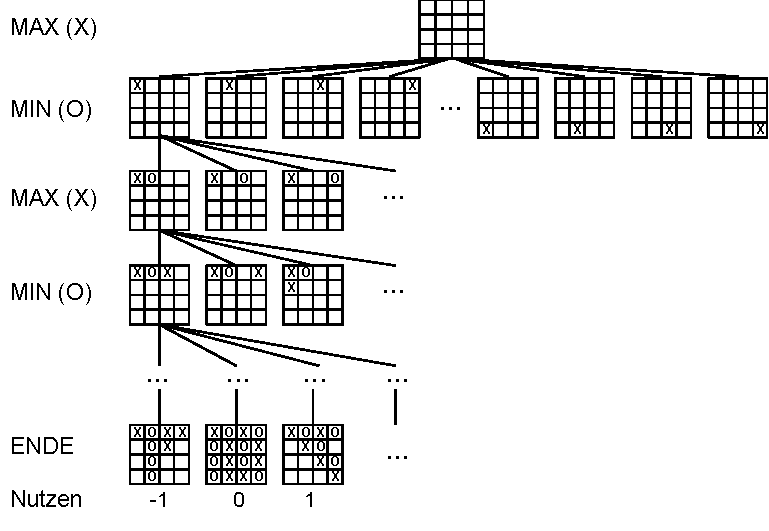
\includegraphics{inhalt/abbildungen/minimax_tictactoe.pdf}
  \caption{Ein (partieller) Suchbaum vgl. \cite[208]{Russell}}
  \label{fig:minimax_tictactoe}
\end{figure} 

Wolfgang Ertel beschreibt in dem nachfolgenden Zitat das Verhältnis von Problemkomplexität und Suchbaumgröße, was belegt, das Suchbäume für Strategiespiele enorme Dimensionen annehmen.\\

''Der effektive Verzweigungsfaktor beim Schachspiel liegt etwa bei 30 bis 35. Bei einem typischen Spiel mit 50 Zügen pro Spieler hat der Suchbaum dann mehr als $30^{100} \approx 10^{148}$ Blattknoten. Der Suchbaum lässt sich also bei weitem nicht vollständig explorieren. Hinzu kommt, dass beim Schachspiel oft mit Zeitbeschränkung gespielt wird. Wegen dieser Realzeitanforderung wird die Tiefe des Suchbaums auf eine passende Tiefe, zum Beispiel acht Halbzüge, beschränkt. \cite[114 \psq]{Ertel}'' \\

\section{Alpha-Beta-Kürzung}
\label{sec:Alpha-Beta-Kürzung}
Eine Möglichkeit die Rechenzeit der Minimax-Suche zu verbessern, ist das Kürzen oder Beschneiden des Suchbaums (eng. Pruning). 

Wolfgang Ertel erklärt die Alpha-Beta Suche wie folgt vgl. \cite[116]{Ertel}:\\
Beim Alpha-Beta-Kürzen wird der Teil des Suchbaums beschnitten, der keinen Effekt auf das Ergebnis der Minimax-Suche hat. Der Minimax Algorithmus wird um zwei Parameter Alpha und Beta ergänzt. Die Bewertung erfolgt an jedem Blattknoten des Suchbaums. Alpha enthält den aktuell größten Wert, für jeden Maximumknoten, der bisher bei der Traversierung (Erkundung oder das Durchlaufen) des Suchbaums gefunden wurde. In Beta wird für jeden Minimumknoten der bisher kleinste gefundene Wert gespeichert. Ist Beta an einem Minimumknoten kleiner oder gleich Alpha ($Beta \leq Alpha$), so kann die Suche unterhalb von diesem Minimumknoten abgebrochen werden. Ist Alpha an einem Maximumknoten größer oder gleich Beta ($Alpha \geq Beta$), so kann die Suche unterhalb von diesem Maximumknoten abgebrochen werden. \\

\begin{figure}[!htbp]
  \centering
  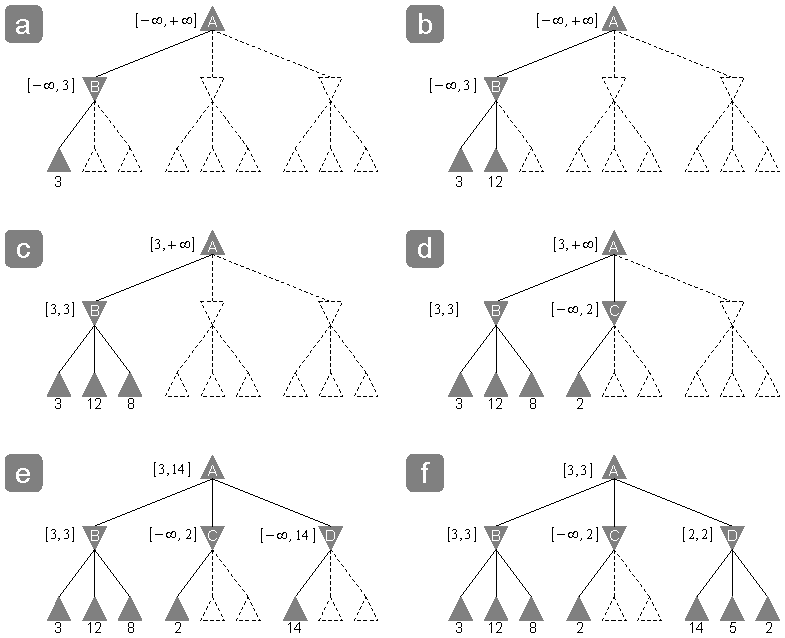
\includegraphics[scale = 0.8]{inhalt/abbildungen/alpha_beta_suchbaum.pdf}
  \caption{Ein Alpha Beta Suchbaum \cite[213]{Russell}.}
  \label{fig:alpha_beta}
\end{figure} 

Verdeutlichen wir das Alpha-Beta-Pruning an Hand eines Beispiels (Abbildung \ref{fig:alpha_beta}). Die nachfolgenden Erklärungen zur Abbildung \ref{fig:alpha_beta} sind in ähnlicher Form in der Literatur zu finden \cite[212 \psqq]{Russell}. Ein Dreieck mit der Spitze nach oben ist ein Maximumknoten und ein Dreieck mit der Spitze nach unten ist ein Minimumknoten. Leere Dreiecke ohne einen bezeichnenden Buchstaben und gestrichelter Umrandung sind noch nicht explorierte Knoten. Durchgängige Linien verweisen auf bereits besuchte Pfade und gestrichelte Linien verweisen auf noch nicht besuchte Pfade. Die Zahlen unterhalb der Blattknoten sind die Nutzwerte, die der maximierende Spieler erhält, wenn er den Pfad bis zu diesem Blattknoten durchschreitet. \\

(a) Minimumknoten B findet einen Nutzwert 3, da dieser Wert der bisher kleinste gefundene Wert ist wird er in Beta gespeichert. \\

(b) Der Minimumknoten B exploriert einen zweiten möglichen Nutzwert 12. Dieser Wert ist höher als der vorher gefundene und in Beta gespeicherte Wert 3, daher wird der minimierende Spieler versuchen diesen Nutzwert für den maximierenden Spieler zu vermeiden. Der neue Wert wird vom Minimumknoten B ignoriert und Beta bleibt unverändert. \\

(c) Minimumknoten B findet den Wert 8, dieser ist genau wie 12 größer als 3 und daher wird Spieler MIN vermeiden, dass Spieler MAX zu diesem Spielergebnis gelangt. Minimumknoten B hat alle seine nachfolgenden Knoten exploriert. Maximumknoten A wird vom Minimumknoten B maximal den Nutzwert 3 erhalten, somit ergibt sich für den Maximumknoten A, dass dieser mindestens den Nutzwert 3 erreichen kann. \\

(d) Ein weiterer Minimumknoten ist C. Der erste Blattknoten von C liefert einen Nutzwert von 2, weil dieser Wert der erste gefundene Wert unterhalb des Minimumknotens C ist, wird er in Beta gespeichert. C wird Maximumknoten A maximal einen Nutzwert 2 liefern. A wiederum kann durch Minimumknoten B bereits einen minimalen Nutzwert von 3 erhalten und hat diesen in Alpha gespeichert. Es gilt $Beta \leq Alpha$ und es ist nicht notwendig die Knoten unterhalb von C weiter zu explorieren. Selbst wenn ein größerer Nutzwert gefunden werden würde, entscheidet sich der minimierende Spieler trotzdem für den kleineren Wert und würde ein kleinerer Nutzwert als 2 gefunden werden, dann entscheidet sich der maximierende Spieler für den Nutzwert 3, den Minimumknoten B liefert. Folglich kann der Suchbaum an dieser Stelle abgeschnitten werden, weil weitere gefundene Nutzwerte keinen Einfluss mehr auf das Ergebnis haben. \\

(e) Der letzte von A zu erreichende Minimumknoten wird exploriert. Der erste Blattknoten unterhalb des Minimumknoten D liefert den Nutzwert 14. Dieser Wert wäre für Maximumknoten A eine starke Verbesserung, weil dieser bisher nur maximal einen Nutzwert von 3 erreichen konnte. Der minimierende Spieler hat noch zwei weitere Möglichkeiten(Knoten) zu explorieren und daher wird er versuchen einen geringeren Nutzwert als 14 zu finden. \\

(f) Minimumknoten D findet in den beiden letzten Blattknoten die Nutzwerte 5 und 2. Der minimierende Spieler wählt die Möglichkeit mit dem geringsten Nutzwert 2. Dieser Nutzwert wird zum neuen Beta Wert. Der Suchbaum wird unterhalb vom Minimumknoten D jedoch nicht abgeschnitten, weil der Nutzwert 2 erst im zuletzt explorierten Knoten gefunden wurde. Theoretisch könnten zwei Pfade unterhalb des Minimumknoten D abgeschnitten werden, wenn der Blattknoten mit dem Nutzwert 2 zuerst exploriert worden wäre.\\

Durch die Alpha-Beta-Kürzung kann ein großer Teil des Suchbaums abgeschnitten werden, ohne das Ergebnis zu beeinflussen. Die Rechenzeit für die Exploration des Suchbaumes, ist an dieser Stelle immer noch zu hoch, deshalb ist eine Suchtiefenbegrenzung erforderlich. Daher wird das Prinzip des Begrenzens der Suchbaumtiefe der iterativ vertiefende Tiefensuche angewendet. \\

\section{Iterativ vertiefende Tiefensuche}
\label{sec:Iterativ vertiefende Tiefensuche}
Um dieses Verfahren zu beschreiben, fassen wir die Ausführungen, zum Thema iterativ vertiefende Tiefensuche, von Russell und Norvig vgl. \cite[116]{Russell} zusammen:\\

Die iterativ vertiefende Tiefensuche (eng. Iterative Deepening) ist ein kombinatorisches, uninformiertes Suchbaumverfahren und kombiniert die Breitensuche mit der Tiefensuche. Die Suchstrategien der uninformierten Suchverfahren haben keine zusätzlichen Informationen über Zustände, außer den in der Problemdefinition vorgegebenen. Alles was sie tun können, ist, Nachfolger zu erzeugen und einen Zielzustand von einem Nichtzielzustand zu unterscheiden. Ein Nachfolger, ist ein Suchbaumknoten, der unterhalb eines anderen Suchbaumknotens existiert. Die Reihenfolge der Suche ist entscheidend für die Unterscheidung der einzelnen uninformierten Suchverfahren. \\
 
Die Breitensuche expandiert (erweitert oder vergrößert) zuerst alle Nachfolger, die in derselben Tiefe liegen, beginnend mit dem Wurzelknoten. Diesen Schritt wiederholt die Breitensuche bis ein gesuchtes Ergebnis gefunden wird oder der Suchbaum vollständig exploriert (erkundet) ist. \\

Die Tiefensuche exploriert zuerst die tiefsten Knoten des Suchbaums (eng. Depth-first). Erreicht die Tiefensuche einen Endknoten, der nicht dem gesuchten Ergebnis entspricht, dann werden die alternativen Knoten, die sich eine Tiefenebene höher befinden, exploriert. \\

Kombinieren wir die uninformierten Suchverfahren Tiefen- und Breitensuche miteinander und mit einer Grenze für die Suchtiefe, erhalten wir die iterative vertiefende Tiefensuche. Diese expandiert zuerst die Nachfolger des Wurzelknotens der Suchtiefe 1. Sind alle Knoten auf dieser Ebene exploriert, dann wird die Schranke für die aktuelle Suchtiefe um 1 erhöht (Iteration) und die Knoten der Suchtiefe 2 werden expandiert. Diese Schritte wiederholt die iterativ vertiefende Tiefensuche bis ein Ziel gefunden wird. \\  

Für diese Arbeit ist dieses Verfahren relevant, weil der vorausschauende Heuristik Agent bzw. die in seiner Implementierung realisierte Alpha-Beta Suche, an die iterativ vertiefende Tiefensuche angepasst wird. Der Agent wird also nicht den gesamten Zustandsraum (Suchbaum) durchsuchen, sondern seine Zugvorausschau wird auf eine bestimmte Anzahl von Zügen begrenzt werden. Meistens wird eine Zugvorausschau von 2 Zügen nicht ausreichen, um einen Blattknoten des Suchbaumes zu erreichen, daher führen wir noch Heuristiken (Bewertungsfunktionen) ein.\\

\section{Heuristik}
\label{sec:Heuristik}
''Heuristiken sind Problemlösungsstrategien, die in vielen Fällen zu einer schnelleren Lösung führen als die uninformierte Suche. Es gibt jedoch keine Garantie hierfür. Die heuristische Suche kann auch viel mehr Rechenzeit beanspruchen und letztlich dazu führen, dass die Lösung nicht gefunden wird. \cite[105]{Ertel}''\\

Wir leiten aus der Definition von Wolfgang Ertel folgendes ab:\\ 
Eine Heuristik (Bewertungsfunktion) berechnet eine Gewinnchance für einen gegebenen Spielzustand, d.h. ob der Spieler in diesem Spielzustand eher gewinnen oder verlieren könnte. Die Verwendung einer Heuristik ist keine Garantie für ein korrektes Ergebnis. In der Regel, wird für bessere Rechenzeit, ein mögliches schlechteres Ergebnis akzeptiert, d.h. eine heuristische Zustandsbewertung muss nicht dem wahren Nutzen des Zustands entsprechen. Die Qualität einer Heuristik ist demnach ausschlaggebend für das Spielergebnis. Ein schlechte Stellungsbewertung (Heuristik), kann schlechte Spielzüge verursachen oder fatale Spielzüge des Gegners übersehen. \\

Die Verwendung einer Heuristik ermöglicht es, Knoten eines Spielbaums zu bewerten, die keine Blattknoten sind. Ohne Heuristiken liefern nur Blattknoten Spielergebnisse und mit Heuristik liefern alle Knoten Spielergebnisse. \\

Wolfgang Ertel schreibt sinngemäß zur Heuristik eines Schachspiels (vgl. \cite[118]{Ertel}): \\
Diese Schach Heuristik ist entstanden aus der Zusammenarbeit von Schachexperten und Wissensingenieuren. Die Schachexperten verfügen über Wissen und Erfahrungen bezüglich des Schachspiels, der Strategien, guter Zugstellungen und schlechter Zugstellungen. Der Wissensingenieur hat die meist sehr schwierige Aufgabe dieses Wissen in eine, für ein Programm, anwendbare Form zu bringen. \\

Eine Bewertungsfunktion B(s) für ein Schachspiel enthält folgende Elemente, wobei s der Parameter für den Spielzustand ist \cite[119]{Ertel}: \\

B(s) = $a_1$ x Material +  $a_2$ x Bauernstruktur + $a_3$ x Königssicherheit \\
\tab \tab + $a_4$ x Springer im Zentrum + $a_5$ x Läufer Diagonalabdeckung + ..., \\ 

das mit Abstand wichtigste Feature (Merkmal) ''Material'' nach der Formel \\

\tab \tab Material = Material(eigenes Team) - Material(Gegner) \\

Material(Team) = Anzahl Bauern(Team) x 100 + Anzahl Springer(Team) x 300 \\
\tab \tab \tab + Anzahl Läufer(Team) x 300 + Anzahl Türme(Team) x 500 \\
\tab \tab \tab + Anzahl Damen(Team) x 900 \\


Nachfolgend liefern wir eine formale, allgemeine Darstellung einer Heuristik. Formal definieren Russell und Norvig Bewertungsfunktionen \cite[218]{Russell}: 

\begin{equation*}
\hat{U}_\theta(s) = \theta_1 f_1(s) + \theta_2 f_2(s) + ... + \theta_n f_n(s),
\end{equation*}

als eine gewichtete Lineare Funktion einer Menge von Merkmalen (oder Basisfunktionen) $f_1, ..., f_n$. Die Parameter $\theta = \theta_1, ... \theta_n$ sind die Gewichtungen der einzelnen Merkmale, d.h. ein Parameter bestimmt, wie ''wichtig'' ein Merkmal ist.

\subsection{Tic Tac Toe Heuristik}
\label{subsec:Tic Tac Toe Heuristik}
Das erste Merkmal unserer Tic Tac Toe Heuristik ist die Kontrolle der mittleren Spielfelder. Spielsituationen in denen die mittleren Spielfelder mit eigenen Spielfiguren besetzt sind, erhalten eine höhere Bewertung. Die erste Spielfigur soll in die mittleren Spielfelder gesetzt werden. Die zweite Spielfigur soll in die vom Gegenspieler nicht gestörte mittlere Position gesetzt werden. \\

\begin{figure}[!htbp]
  \centering
  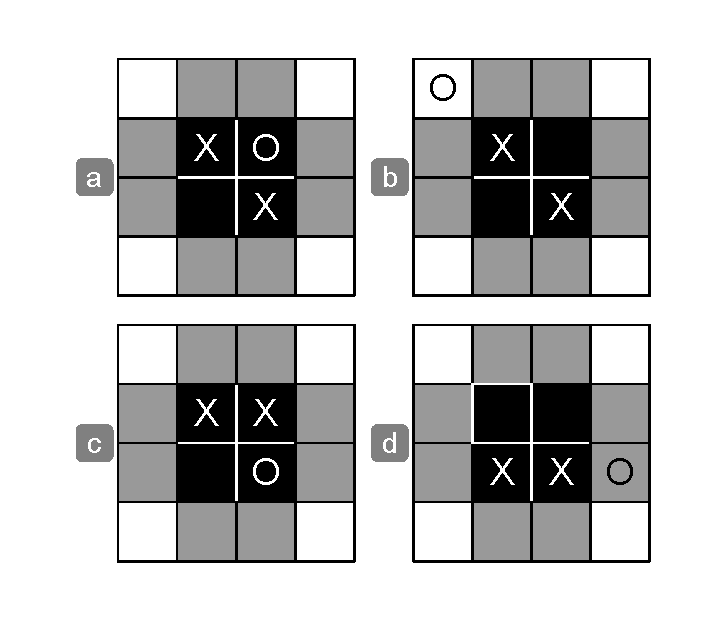
\includegraphics[scale = 0.5]{inhalt/abbildungen/tictactoe_mid_control.pdf}
  \caption{Tic Tac Toe Eröffnungssituationen.}
  \label{fig:tictactoe_mid_control}
\end{figure}

Abbildung \ref{fig:tictactoe_mid_control} zeigt 4 verschiedene Spielsituationen. Wir werden das erste Merkmal der Tic Tac Toe Heuristik an diesem Beispiel erklären. Spielsituation (a) wird, nach der Definition des ersten Merkmals, eine bessere heuristische Bewertung erhalten, als Spielsituation (b). Die Kreuzspielsteine sind in beiden Spielsituationen zwar gleich positioniert, aber der Kreisspielstein stört in Spielsituation (b) die Siegesformation des Kreuzspielers. Aus dem selben Grund ist Spielsituation (c) ''wertvoller'' oder ''nützlicher'' als Spielsituation (d). In Spielsituation (c) ist eine mögliche Siegesformation des Kreuzspielers (mit bereits 2 Kreuzfiguren) ungestört. In Spielsituation (d) ist die diagonale Siegesformation des Kreuzspielers bereits gestört und somit unbrauchbar, hinsichtlich einer größeren Gewinnchance. \\

Das zweite Merkmal der Tic Tac Toe Heuristik ist die Beachtung der ungestörten Möglichkeiten für Siegesformationen. Eine Formationsmöglichkeit wird gefährlicher bzw. attraktiver, je mehr gleiche Spielfiguren sich bereits in dieser befinden. Wir stellen bei diesem Merkmal gegenüber, wie viele, vom Gegenspieler nicht gestörte Formationsmöglichkeiten  einem Spieler zur Verfügung stehen. Gleichzeitig berücksichtigen wir, wie viele ungestörte Formationsmöglichkeiten der Gegenspieler hat. \\

\begin{figure}[!htbp]
  \centering
  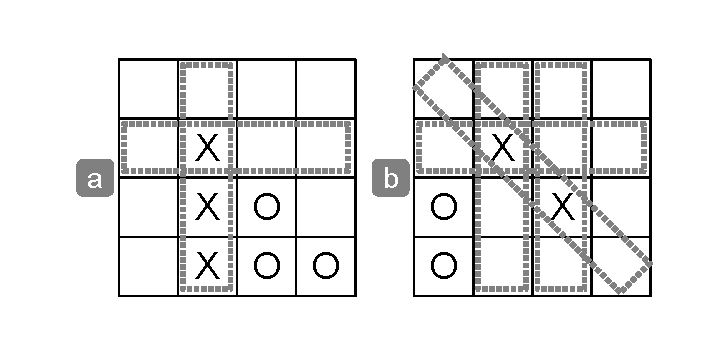
\includegraphics[scale = 0.7]{inhalt/abbildungen/tictactoe_formations.pdf}
  \caption{Tic Tac Toe Formationsmöglichkeiten.}
  \label{fig:tictactoe_formations}
\end{figure}

Betrachten wir die ungestörten möglichen Siegesformationen in Abbildung \ref{fig:tictactoe_formations}. In Spielsituation (a) hat der Kreuzspieler 2 Möglichkeiten eine Siegesformation zu erreichen. In der vertikalen Formation sind bereits 3 Kreuze und in der diagonalen 1 Kreuz vorhanden. Die vertikal mögliche Siegesformation ist wesentlich hochwertiger, als die diagonal mögliche Siegesformation, weil diese bereits mehr Kreuzfiguren enthält. In Spielsituation (b) verfügt der Kreuzspieler über 4 mögliche ungestörte Siegesformationen, wobei die diagonal mögliche Siegesformation attraktiver sein sollte, als die anderen 3 möglichen Formationen. Die möglichen Siegesformationen des Gegenspielers sollen ebenfalls berücksichtigt werden.

\subsection{Reversi Heuristik}
\label{subsec:Reversi Heuristik}
Für die Erstellung der Reversi Heuristik verwenden wir bereits existierendes strategisches Wissen (siehe Sammlung von Reversi Strategien \cite{MacGuire}). \\

Das erste wichtige Merkmal für unsere Reversi Heuristik ist die Mobilität. Das Merkmal der Mobilität wird in zwei Merkmale aufgeteilt. Ein Merkmal für die aktuelle Mobilität und ein zweites Merkmal für die mögliche Mobilität. Mit aktueller Mobilität ist die Anzahl aller möglichen Spielzüge in einem aktuellen Spielzustand gemeint. Die Anzahl der Spielsteine am Ende des Spiels ist zwar entscheidend, aber in den Spielzügen bevor das Spiel endet, ist der Spieler im Vorteil, der mehr Zugmöglichkeiten hat. \\

Abbildung \ref{fig:reversi_maximum_disk_strategy} zeigt eine Spielsituation in der Spieler Weiß nahezu alle Spielsteine kontrolliert. Spieler Schwarz ist jedoch der einzige Spieler der noch über Mobilität verfügt, d.h. er kann noch Spielzüge ausführen. In den nachfolgenden 4 Spielzügen $(0,0) \rightarrow (0,7) \rightarrow (7,0) \rightarrow (7,7)$ gewinnt der Schwarze Spieler die Partie. \\

\begin{figure}[!htbp]
  \centering
  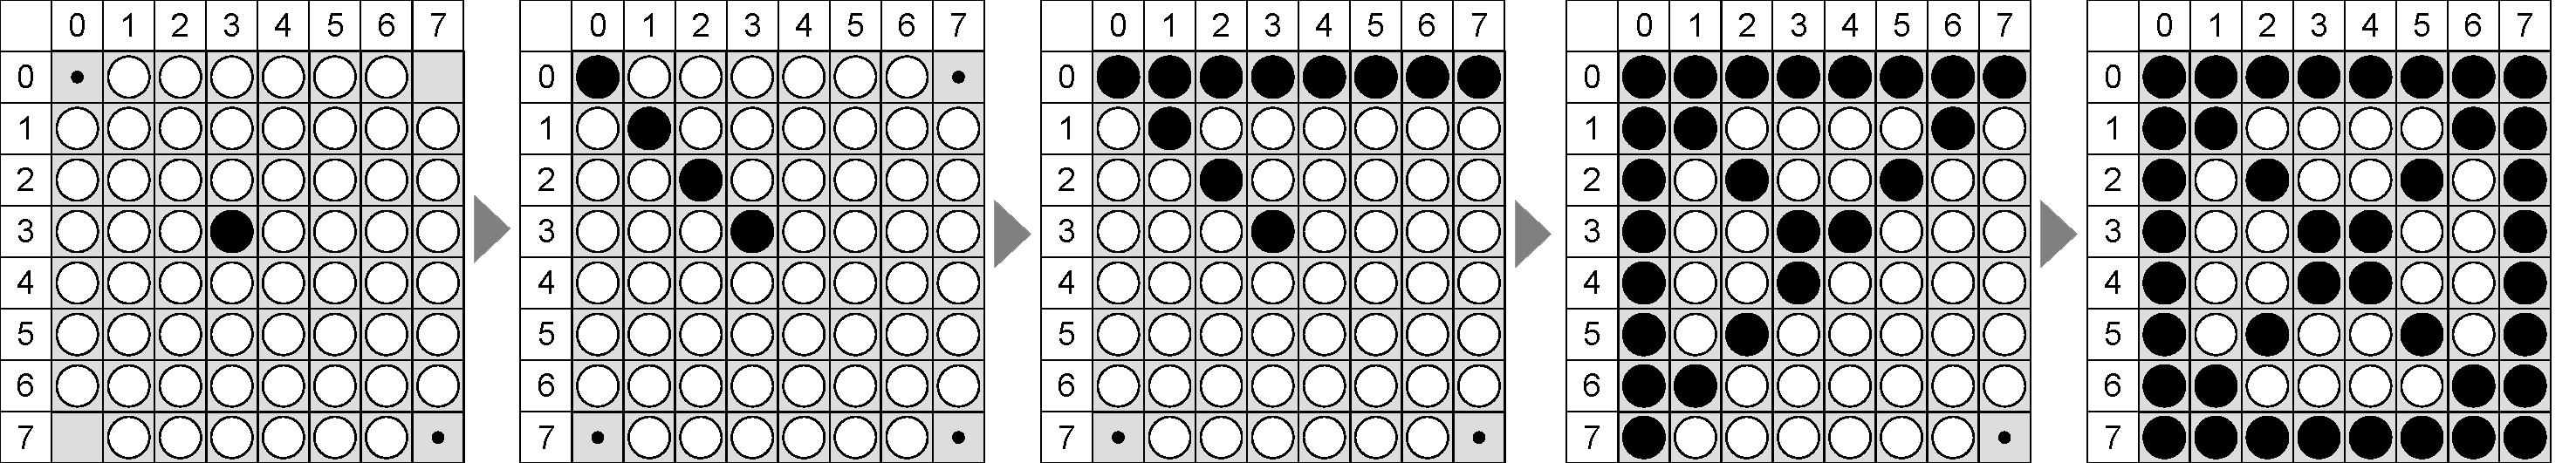
\includegraphics[scale = 0.3]{inhalt/abbildungen/reversi_maximum_disk_strategy.pdf}
  \caption{Reversi Merkmal der aktuellen Mobilität.}
  \label{fig:reversi_maximum_disk_strategy}
\end{figure}

Die mögliche Mobilität beachtet alle freien Spielfelder, die an gegnerische Spielsteine Angrenzen. In Abbildung \ref{fig:reversi_movement_notation_positioning} (a) ist Spieler Weiß am Zug. Die aktuelle Mobilität ist in dieser Spielsituation identisch mit der möglichen Mobilität, denn es gibt nur 3 freie Spielfelder die an schwarze Spielsteine angrenzen. Bei der ersten Spielsituation in Abbildung \ref{fig:reversi_maximum_disk_strategy} ist die aktuelle Mobilität gleich 2 und die mögliche Mobilität gleich 4.\\

Das zweite wichtige Merkmal für unsere Reversi Heuristik ist die Bewertung der Eckspielfelder und der Randspielfelder. In Abbildung \ref{fig:reversi_movement_notation_positioning} (b) sind bestimmte Spielfelder mit Buchstaben gekennzeichnet, diese Buchstaben repräsentieren Spielfelder mit bestimmten Eigenschaften. Alle X-Spielfelder (eng. x-squares) sollten unbedingt vermieden werden, denn sie bieten dem Gegner (fast immer) die Möglichkeit eine der 4 Ecken zu besetzen. Es existieren auch Strategien, die die vier Ecken generell, aus Gründen eingeschränkter Mobilität, vermeiden. \\

Das Ziel unserer Reversi Heuristik soll das Besetzen dieser 4 Ecken sein und gleichzeitig das Verhindern, dass der Gegenspieler diese Ecken besetzt. Genau wie die X-Spielfelder, bieten die C-Spielfelder direkten Zugang zu den 4 Ecken des Spielbretts. Die C-Spielfelder sollen daher ebenfalls vermieden werden. A- und B-Spielfelder sind zu bevorzugen und können besetzt werden. In Abbildung \ref{fig:reversi_movement_notation_positioning} (c) sind die einzelnen Bewertungen der Positionen veranschaulicht. Diese numerischen Bewertungen beziehen sich auf das gesamte Reversi Spielbrett, weil dieses symmetrisch ist.


\begin{figure}[!htbp]
  \centering
  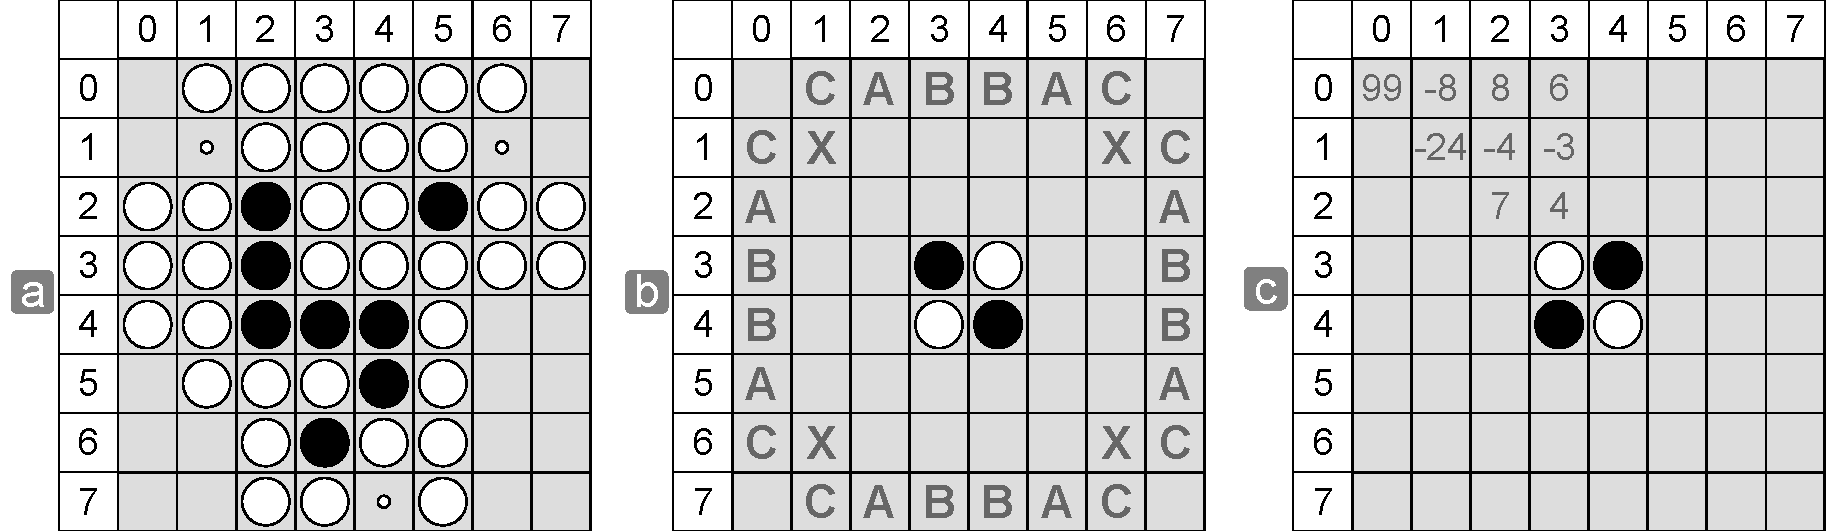
\includegraphics[scale = 0.5]{inhalt/abbildungen/reversi_movement_notation_positioning.pdf}
  \caption{Merkmale einer Reversi Heuristik.}
  \label{fig:reversi_movement_notation_positioning}
\end{figure}
